\documentclass[11pt, a4paper]{article}
\usepackage[utf8]{inputenc}
\usepackage[T1]{fontenc}
\usepackage[english]{babel}
\usepackage{geometry}
\usepackage{booktabs}
\usepackage{hyperref}
\usepackage{lmodern}
\usepackage{graphicx}
\usepackage{amsmath} % For math equations and \text command
\usepackage{amssymb} % For checkmark and math symbols
\usepackage[table]{xcolor} % Ajout pour la couleur des tableaux
\usepackage{pgfplots} % Ajout pour les graphiques
\usepackage{soul} % For text highlighting
\usepackage{fancyhdr} % For custom headers and footers
\usepackage{tcolorbox} % For callout boxes
\usepackage{multicol} % For two-column layout
\pgfplotsset{compat=1.18} % Spécifier une version de compatibilité

% Couleurs personnalisées (consistent severity palette)
\definecolor{lightgreen}{rgb}{0.85,1,0.85}
\definecolor{lightorange}{rgb}{1,0.9,0.8}
\definecolor{lightred}{rgb}{1,0.8,0.8}
\definecolor{vuln-critical}{rgb}{0.8,0.1,0.1}  % Dark red
\definecolor{vuln-high}{rgb}{1,0.4,0}          % Orange
\definecolor{vuln-medium}{rgb}{1,0.8,0}        % Yellow
\definecolor{vuln-low}{rgb}{0.4,0.6,0.9}       % Light blue
\definecolor{gantt-supported}{rgb}{0.2,0.7,0.3}
\definecolor{gantt-eol}{rgb}{0.8,0.2,0.2}
\definecolor{highlight}{rgb}{1,1,0.7}          % Light yellow for highlighting


% Configuration des marges
\geometry{a4paper, margin=1in}

% Configuration des liens hypertextes
\hypersetup{
    colorlinks=true,
    linkcolor=blue,
    urlcolor=blue,
    pdftitle={PostgreSQL Security Analysis},
    pdfauthor={Adrien SALES (@rastadidi)},
    pdfsubject={Security, PostgreSQL, Vulnerabilities, DevOps},
    pdfkeywords={PostgreSQL, security, vulnerability, DevOps, DevSecOps, SecOPS, docker, trivy, geol}
}

% Titre et auteur
\title{PostgreSQL Security Analysis\\ \large with \texttt{geol} and \texttt{trivy} tools \\ github.com/adriens/geol-showcase}
\author{Gemini CLI | \texttt{geol} | \texttt{trivy} | Adrien SALES ($\mathbf{X}$ \texttt{@rastadidi})}
\date{\today}

% Configure footer with generation metadata
\pagestyle{fancy}
\fancyhf{} % Clear default headers/footers
\fancyhead[L]{\small PostgreSQL Security Analysis}
\fancyhead[R]{\small\thepage}
\fancyfoot[C]{\footnotesize Generated with \texttt{geol} 2.7.1, \texttt{trivy} 0.69.1, \texttt{gemini-cli} 0.28.2 on \today}
\renewcommand{\headrulewidth}{0.4pt}
\renewcommand{\footrulewidth}{0.4pt}

% Plain style for first page
\fancypagestyle{plain}{
  \fancyhf{}
  \fancyfoot[C]{\footnotesize Generated with \texttt{geol} 2.7.1, \texttt{trivy} 0.69.1, \texttt{gemini-cli} 0.30.0 on \today}
  \renewcommand{\headrulewidth}{0pt}
  \renewcommand{\footrulewidth}{0.4pt}
}

\begin{document}

\maketitle

\begin{abstract}
This article presents a concise analysis of the security and lifecycle of
the \href{https://www.postgresql.org/}{PostgreSQL} database versions.

Using the \href{https://github.com/opt-nc/geol}{\texttt{geol}} tool to check End-of-Life dates and \href{https://trivy.dev/}{\texttt{trivy}} to scan vulnerabilities in official Docker images, I establish a risk profile for currently supported and unsupported versions.\\

The goal is to demonstrate the crucial importance of using maintained versions and the value of combining generative AI with optimally designed CLI tools to automate and enrich this type of analysis.
\end{abstract}

\tableofcontents
\newpage

% ============================================
% EXECUTIVE ONE-PAGER
% ============================================
\section*{Executive One-Pager}
\addcontentsline{toc}{section}{Executive One-Pager}

\begin{center}
\Large\textbf{PostgreSQL Security Status At-a-Glance}\\
\normalsize Data as of \today
\end{center}

\vspace{0.5cm}

\begin{center}
\begin{tabular}{cc}
\begin{minipage}{0.45\textwidth}
\begin{tcolorbox}[colback=lightgreen, colframe=gantt-supported, title=\textbf{✓ Supported Versions}, fonttitle=\bfseries]
\centering
\Huge\textbf{5}\\
\normalsize Versions 14-18\\[0.3cm]
\large\textbf{0-1} Critical CVEs\\
\large\textbf{6-17} High CVEs\\[0.2cm]
\small Risk Score: \textbf{146-275}\\
\textcolor{gantt-supported}{\textbf{LOW RISK}}
\end{tcolorbox}
\end{minipage}
&
\begin{minipage}{0.45\textwidth}
\begin{tcolorbox}[colback=lightred, colframe=gantt-eol, title=\textbf{✗ End-of-Life Versions}, fonttitle=\bfseries]
\centering
\Huge\textbf{5}\\
\normalsize Versions 9.6-13\\[0.3cm]
\large\textbf{7-10} Critical CVEs\\
\large\textbf{70-97} High CVEs\\[0.2cm]
\small Risk Score: \textbf{643-764}\\
\textcolor{vuln-critical}{\textbf{HIGH RISK}}
\end{tcolorbox}
\end{minipage}
\end{tabular}
\end{center}

\vspace{0.5cm}

\subsection*{Critical Decision Matrix}

\begin{center}
\begin{tabular}{|l|l|c|}
\hline
\rowcolor{lightgray}
\textbf{If Your Version Is...} & \textbf{Action Required} & \textbf{Risk Score} \\ \hline
\rowcolor{lightred} ≤ 13 (EOL) & \textbf{URGENT}: Migrate immediately (2-10$\times$ more vulnerabilities) & 643-764 \\ \hline
\rowcolor{lightorange} 14 & Plan upgrade to 16/17 (EOL approaching 2026) & 146 \\ \hline
\rowcolor{lightgreen} 15-17 & Monitor for patches, review annually & 146 \\ \hline
\rowcolor{lightgreen} 18 (Latest) & Excellent - maintain patch currency & 275 \\ \hline
\end{tabular}
\end{center}

\vspace{0.5cm}

\subsection*{Key Metrics Summary}

\begin{multicols}{2}
\begin{itemize}
    \item \textbf{Vulnerability Reduction}: Upgrading from v12 to v17 eliminates \textbf{9 critical CVEs} and reduces total vulnerabilities by \textbf{63\%}
    \item \textbf{Risk Score Improvement}: v12→v17 reduces risk score from \textbf{764 to 146} (81\% reduction)
    \item \textbf{Patch Effectiveness}: v18.0→v18.1 reduced risk score by \textbf{36\%} (428→275)
    \item \textbf{Support Window}: 5-year lifecycle per major version
    \item \textbf{Latest Supported}: Version 18 (EOL: Nov 2030)
    \item \textbf{Next EOL Event}: Version 14 (Nov 2026)
    \item \textbf{Tools Used}: \texttt{geol} 2.7.1, \texttt{trivy} 0.69.1, \texttt{gemini-cli} 0.30.0
\end{itemize}
\end{multicols}

\vspace{0.5cm}

\begin{tcolorbox}[colback=lightorange!30, colframe=vuln-high, title=⚠️ Immediate Action Required, fonttitle=\bfseries]
\textbf{If running PostgreSQL ≤13:}
\begin{enumerate}
    \item Run \texttt{geol check} to verify EOL status
    \item Scan images: \texttt{trivy image postgres:X}
    \item Plan migration to version ≥14 within 30 days
    \item Review Section \ref{sec:recommendations} for detailed upgrade paths
\end{enumerate}
\end{tcolorbox}

\vspace{0.3cm}

\begin{center}
\textit{Full analysis with charts, CVE details, and migration strategies follows...}
\end{center}

\newpage

\section{Executive Summary}

\textbf{Key Findings:}

\begin{itemize}
    \item \textbf{\textcolor{gantt-supported}{5 Supported Versions:}} PostgreSQL versions 14-18 are actively maintained with EOL dates ranging from 2026 to 2030.
    \item \textbf{\textcolor{gantt-eol}{Fresh EOL Alert:}} PostgreSQL 13 recently reached end-of-life on November 13, 2025, joining versions 9.6-12 as unsupported.
    \item \textbf{\textcolor{vuln-critical}{Security Gap:}} Unsupported versions contain \textbf{\textcolor{vuln-critical}{2-10$\times$ more vulnerabilities}} than supported versions, with critical CVEs present only in EOL versions.
    \item \textbf{Patch Impact:} Minor updates are crucial - PostgreSQL 18.1 reduced vulnerabilities by \textbf{\textcolor{gantt-supported}{22\%}} compared to 18.0 (204 → 159 total vulnerabilities).
    \item \textbf{\textcolor{vuln-critical}{Critical Recommendation:}} Migrate immediately from any version $\leq$13 to version $\geq$14. The security risk of unsupported versions is unacceptable for production environments.
\end{itemize}

\textbf{Risk Profile Summary:}
\begin{itemize}
    \item $\checkmark$ \textbf{\textcolor{gantt-supported}{Low Risk:}} Versions 14-18 (0-1 critical, 6-17 high vulnerabilities)
    \item $\times$ \textbf{\textcolor{gantt-eol}{High Risk:}} Versions 9.6-13 (7-10 critical, 70-97 high vulnerabilities)
\end{itemize}

\section{Introduction to the Tools}

Maintaining a secure software infrastructure relies on two fundamental pillars:

\begin{itemize}
    \item \textbf{Actively supported versions}
    \item \textbf{Awareness of vulnerabilities} present in the components we deploy
\end{itemize}

Below is a quick overview of the tools used for this analysis.

\subsection{\texttt{geol}: The Lifecycle Guardian}

\href{https://github.com/opt-nc/geol}{\texttt{geol}} (version 2.7.1) is a tool that queries the \href{https://endoflife.date}{endoflife.date} API to instantly retrieve software End-of-Life dates.

\subsection{\texttt{trivy}: The Vulnerability Scanner}
\href{https://trivy.dev/}{\texttt{trivy}} (version 0.69.1) is an open-source scanner that detects vulnerabilities (CVEs) in container images, file systems, and Git repositories. The vulnerability database is version 2.

\subsection{\texttt{gemini-cli}: AI Assistant}
\href{https://github.com/google-gemini/gemini-cli}{\texttt{gemini-cli}} (version 0.30.0) is an open-source AI agent that brings Gemini's power directly to the terminal.

\subsection{\LaTeX{}: Report Generator}

\LaTeX{} is a document composition system that produces high-quality technical and scientific reports. We use \texttt{xelatex} for compilation. It is particularly suited for structuring, formatting, and presenting security analysis results clearly and professionally.

\section{PostgreSQL Overview}

PostgreSQL \href{https://www.postgresql.org/}{https://www.postgresql.org/}, also known as Postgres, is a free and open-source relational database management system (RDBMS) emphasizing extensibility and technical standards compliance.

Postgres recommends that all users run the latest available minor release for whatever major version is in use.

The PostgreSQL Global Development Group supports a major version for 5 years after its initial release. After its five-year anniversary, a major version will have one last minor release containing any fixes and will be considered end-of-life (EOL) and no longer supported.

The Release roadmap \href{https://www.postgresql.org/developer/roadmap/}{https://www.postgresql.org/developer/roadmap/} lists upcoming minor and major releases. If the release team determines that a critical bug or security fix is too important to wait until the regularly scheduled minor release, it may make a release available outside the minor release roadmap.

A Feature Matrix \href{https://www.postgresql.org/about/featurematrix/}{https://www.postgresql.org/about/featurematrix/} documents feature availability against major releases.

\section{Methodology}

The analysis for this report was conducted on \today. The data was gathered using the following open-source tools and commands:

\begin{itemize}
    \item \textbf{Lifecycle Data:} PostgreSQL version lifecycle information was retrieved using the \texttt{geol} CLI with the command:
    \begin{verbatim}
        geol product extended psql -n0
    \end{verbatim}
    \item \textbf{Vulnerability Scanning:} Docker images for each major PostgreSQL version were scanned for vulnerabilities using the \texttt{trivy} CLI. An example command for a single version is:
    \begin{verbatim}
        trivy image postgres:18
    \end{verbatim}
\end{itemize}

\subsection{Trivy Scanning Techniques and Data Extraction}

To efficiently aggregate vulnerability data from \texttt{trivy} scans, several command-line techniques were employed. This section details the practical scripts and \texttt{jq} tricks used to extract and count vulnerabilities by severity.

\subsubsection{Method 1: Template-Based Extraction}

The most efficient approach uses \texttt{trivy}'s built-in template engine to extract only severity information:

\begin{verbatim}
trivy image --format template \
  --template '{{- range . -}}{{- range .Vulnerabilities -}}
{{ .Severity }}{{ "\n" }}{{- end -}}{{- end -}}' \
  postgres:18.3 2>/dev/null | sort | uniq -c
\end{verbatim}

\noindent This command:
\begin{itemize}
    \item Uses \texttt{-{}-format template} to customize output
    \item Iterates through all vulnerabilities with nested \texttt{range} loops
    \item Extracts only the \texttt{.Severity} field
    \item Redirects stderr to \texttt{/dev/null} to suppress progress messages
    \item Pipes to \texttt{sort | uniq -c} to count occurrences by severity
\end{itemize}

\noindent Example output:
\begin{verbatim}
      1 CRITICAL
     16 HIGH
     39 MEDIUM
    111 LOW
\end{verbatim}

\subsubsection{Method 2: JSON Output with jq}

For more complex data extraction, \texttt{trivy} can output full JSON which is then processed with \texttt{jq}:

\begin{verbatim}
trivy image postgres:18.3 --quiet --format json | \
  jq -r '.Results[]?.Vulnerabilities[]?.Severity' | \
  sort | uniq -c
\end{verbatim}

\noindent This approach:
\begin{itemize}
    \item Uses \texttt{-{}-format json} for structured output
    \item \texttt{jq -r} extracts raw severity values without quotes
    \item \texttt{.Results[]?} safely iterates through all result objects
    \item \texttt{.Vulnerabilities[]?} accesses the vulnerabilities array
    \item The \texttt{?} operator prevents errors if fields are missing
\end{itemize}

\subsubsection{Method 3: Detailed CVE Information}

To extract specific CVE details (ID, severity, description):

\begin{verbatim}
trivy image postgres:12 --quiet --format json | \
  jq -r '.Results[].Vulnerabilities[] | 
    select(.Severity == "CRITICAL") | 
    "\(.VulnerabilityID): \(.Title)"'
\end{verbatim}

\noindent This extracts only critical vulnerabilities with their titles, useful for the CVE examples table.

\subsubsection{Method 4: Risk Score Calculation}

To calculate the risk score directly from \texttt{trivy} output:

\begin{verbatim}
trivy image postgres:18.3 --quiet --format json | \
  jq '[.Results[].Vulnerabilities[] | .Severity] | 
    (map(select(. == "CRITICAL")) | length) * 10 + 
    (map(select(. == "HIGH")) | length) * 5 + 
    (map(select(. == "MEDIUM")) | length) * 2 + 
    (map(select(. == "LOW")) | length) * 1'
\end{verbatim}

\noindent This single command:
\begin{itemize}
    \item Extracts all severity values into an array
    \item Counts each severity level
    \item Applies the weighted formula: $10 \times \text{Critical} + 5 \times \text{High} + 2 \times \text{Medium} + 1 \times \text{Low}$
    \item Returns the final risk score
\end{itemize}

\subsubsection{Scanning Multiple Versions in Batch}

To scan all PostgreSQL versions efficiently:

\begin{verbatim}
for version in 18.3 17 16 15 14 13 12 11 10 9.6; do
  echo -n "postgres:$version - "
  trivy image --format template \
    --template '{{- range . -}}{{- range .Vulnerabilities -}}
{{ .Severity }}{{ "\n" }}{{- end -}}{{- end -}}' \
    postgres:$version 2>/dev/null | \
    awk '{crit+=($1=="CRITICAL"); high+=($1=="HIGH"); 
         med+=($1=="MEDIUM"); low+=($1=="LOW")} 
         END {print "C:"crit" H:"high" M:"med" L:"low}'
done
\end{verbatim}

\noindent This loop processes all versions and outputs a compact summary.

\subsubsection{Docker Image Digest Verification}

To ensure reproducible scans, images can be referenced by their manifest digest:

\begin{verbatim}
trivy image postgres:18.3@sha256:eb37f58646a901dc7727cf448... 
\end{verbatim}

\noindent Using digests guarantees scanning the exact same image, even if tags are updated.

\begin{tcolorbox}[colback=lightgreen!20, colframe=gantt-supported, title=💡 Best Practices for Vulnerability Scanning, fonttitle=\bfseries]
\begin{itemize}
    \item Use \texttt{-{}-quiet} to suppress progress output in scripts
    \item Redirect stderr (\texttt{2>/dev/null}) when using template output
    \item Reference images by digest for reproducible CI/CD scans
    \item Cache \texttt{trivy} database updates to speed up batch scans
    \item Use \texttt{-{}-severity CRITICAL,HIGH} to focus on high-priority issues
    \item Integrate into pre-deployment gates with \texttt{-{}-exit-code 1}
\end{itemize}
\end{tcolorbox}

\newpage

\section{Data Analysis}

\subsection{Version Lifecycle (\texttt{geol} data)}

The first step is to determine which versions are officially supported.\\

An unsupported version is a \textbf{gateway to unpatched vulnerabilities.}

\begin{table}[htbp]
\centering
\caption{PostgreSQL Version Lifecycle}
\label{tab:geol}
\begin{tabular}{@{}lccccl@{}}
	
	\textbf{Version} & \textbf{Release Date} & \textbf{Latest} & \textbf{Latest Release} & \textbf{End of Support (EOL)} & \textbf{Status} \\ \midrule
\rowcolor{lightgreen} 18 & 2025-09-25 & 18.3 & 2026-02-23 & 2030-11-14 & $\checkmark$ Supported \\
\rowcolor{lightgreen} 17 & 2024-09-26 & 17.9 & 2026-02-23 & 2029-11-08 & $\checkmark$ Supported \\
\rowcolor{lightgreen} 16 & 2023-09-14 & 16.13 & 2026-02-23 & 2028-11-09 & $\checkmark$ Supported \\
\rowcolor{lightgreen} 15 & 2022-10-13 & 15.17 & 2026-02-23 & 2027-11-11 & $\checkmark$ Supported \\
\rowcolor{lightgreen} 14 & 2021-09-30 & 14.22 & 2026-02-23 & 2026-11-12 & $\checkmark$ Supported \\
\rowcolor{lightred} 13 & 2020-09-24 & 13.23 & 2025-11-10 & 2025-11-13 & $\times$ \textbf{Unsupported} \\ \midrule
\rowcolor{lightred} 12 & 2019-10-03 & 12.22 & 2024-11-18 & 2024-11-21 & $\times$ \textbf{Unsupported} \\
\rowcolor{lightred} 11 & 2018-10-18 & 11.22 & 2023-11-06 & 2023-11-09 & $\times$ \textbf{Unsupported} \\
\rowcolor{lightred} 10 & 2017-10-05 & 10.23 & 2022-11-07 & 2022-11-10 & $\times$ \textbf{Unsupported} \\
\rowcolor{lightred} 9.6 & 2016-09-29 & 9.6.24 & 2021-11-08 & 2021-11-11 & $\times$ \textbf{Unsupported} \\ \bottomrule
\end{tabular}
\end{table}


\subsection{Vulnerability Analysis (\texttt{trivy} data)}

The second step is to analyze the "attack surface" of Docker images. It's important to note that while we use major version Docker tags (e.g., \texttt{postgres:18}), these tags typically point to the latest patch release within that major version series (e.g., \texttt{postgres:18} currently refers to \texttt{postgres:18.1}).

\subsubsection{Risk Scoring Methodology}

To quantify the security risk of each PostgreSQL version, we apply a weighted risk scoring formula that prioritizes critical and high-severity vulnerabilities:

\begin{equation}
\boxed{
\text{Risk Score} = \sum_{i} w_i \cdot n_i = 10 \cdot n_{\text{Critical}} + 5 \cdot n_{\text{High}} + 2 \cdot n_{\text{Medium}} + 1 \cdot n_{\text{Low}}
}
\end{equation}

\noindent where $n_i$ represents the number of vulnerabilities at each severity level, and $w_i$ are the corresponding weights reflecting the relative security impact.

\vspace{0.3cm}

\noindent\textbf{Risk Classification with Severity Overrides:}

To prevent misclassification of versions with few but critical vulnerabilities, we apply severity-based override rules:

\begin{equation}
\boxed{
\text{Risk Level} = 
\begin{cases}
\textcolor{vuln-critical}{\textbf{High}} & \text{if } \text{Score} > 300 \text{ OR } n_{\text{Critical}} \geq 3 \\[0.3cm]
\textcolor{vuln-medium}{\textbf{Medium}} & \text{if } 150 \leq \text{Score} \leq 300 \text{ OR } n_{\text{Critical}} \geq 1 \\[0.3cm]
\textcolor{gantt-supported}{\textbf{Low}} & \text{if } \text{Score} < 150 \text{ AND } n_{\text{Critical}} = 0
\end{cases}
}
\end{equation}

\vspace{0.2cm}

\noindent This ensures that:
\begin{itemize}
    \item Any version with 3+ critical CVEs is \textbf{automatically High Risk}, regardless of score
    \item Any version with 1+ critical CVE is \textbf{at least Medium Risk}
    \item Only versions with \textbf{zero critical CVEs} can achieve Low Risk status
\end{itemize}

Table \ref{tab:trivy} and Figure \ref{fig:vuln-chart} show the results.

\begin{tcolorbox}[colback=lightred!30, colframe=vuln-critical, title=⚠️ Critical Finding: EOL Version Vulnerability Gap, fonttitle=\bfseries]
\textbf{Unsupported versions (9.6-13) contain 2-10$\times$ more vulnerabilities than supported versions (14-18).} PostgreSQL 12 alone has a \textbf{risk score of 764} (High Risk) with \textbf{9 critical CVEs}, compared to a score of \textbf{146} (Low Risk) and \textbf{0 critical} in version 17.
\end{tcolorbox}

\begin{table}[htbp]
\centering
\caption{Vulnerability Summary by Version with Risk Scores}
\label{tab:trivy}
\begin{tabular}{@{}lcccccc@{}}
	\textbf{Docker Tag} & \textbf{Critical} & \textbf{High} & \textbf{Medium} & \textbf{Low} & \textbf{Total} & \textbf{Risk Score} \\ \midrule
\rowcolor{lightorange} \texttt{postgres:18.3} & 1 & 16 & 39 & 111 & 167 & \textbf{269} \\
\rowcolor{lightorange} \texttt{postgres:18.2} & 1 & 16 & 39 & 111 & 167 & \textbf{269} \\
\rowcolor{lightgreen} \texttt{postgres:17} & 0 & 6 & 9 & 98 & 113 & \textbf{146} \\
\rowcolor{lightgreen} \texttt{postgres:16} & 0 & 6 & 9 & 98 & 113 & \textbf{146} \\
\rowcolor{lightgreen} \texttt{postgres:15} & 0 & 6 & 9 & 98 & 113 & \textbf{146} \\
\rowcolor{lightgreen} \texttt{postgres:14} & 0 & 6 & 9 & 98 & 113 & \textbf{146} \\
\rowcolor{lightgreen} \texttt{postgres:13} & 0 & 6 & 9 & 98 & 113 & \textbf{146} \\ \midrule
\rowcolor{lightred} \texttt{postgres:12} & 9 & 70 & 100 & 124 & 305 & \textbf{764} \\
\rowcolor{lightred} \texttt{postgres:11} & 7 & 84 & 52 & 49 & 192 & \textbf{643} \\
\rowcolor{lightred} \texttt{postgres:10} & 7 & 84 & 52 & 49 & 192 & \textbf{643} \\
\rowcolor{lightred} \texttt{postgres:9.6} & 10 & 97 & 57 & 49 & 213 & \textbf{748} \\ \bottomrule
\end{tabular}
\end{table}

\begin{figure}[htbp]
\centering
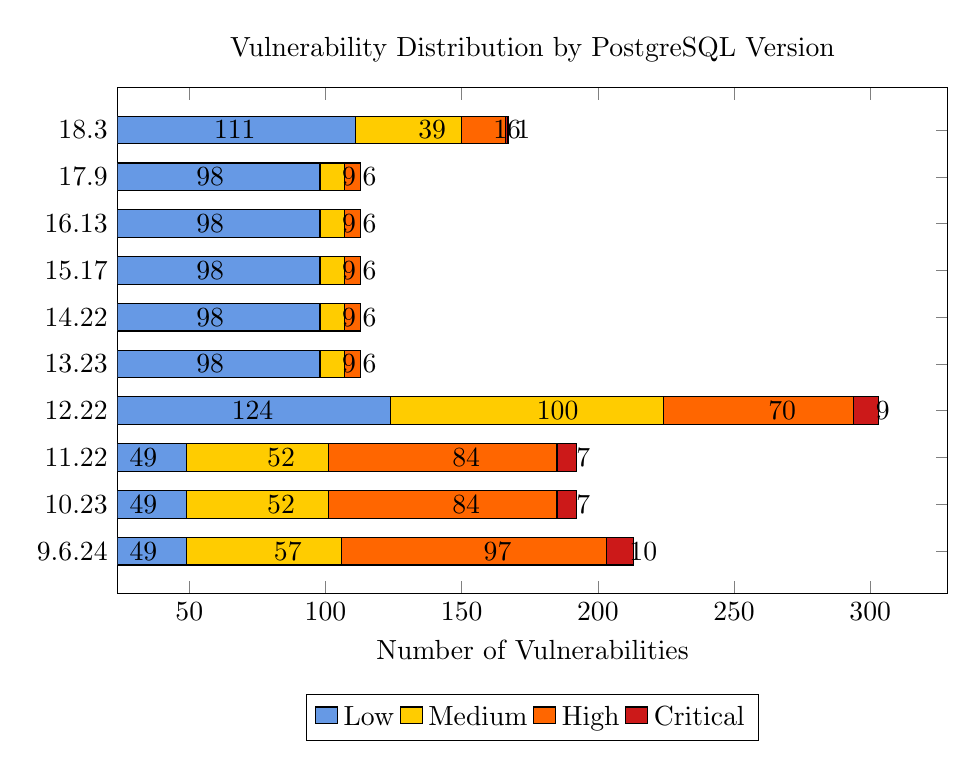
\begin{tikzpicture}
\begin{axis}[
    xbar stacked,
    width=\textwidth,
    height=8cm,
    title={Vulnerability Distribution by PostgreSQL Version},
    xlabel={Number of Vulnerabilities},
    symbolic y coords={9.6.24, 10.23, 11.22, 12.22, 13.23, 14.22, 15.17, 16.13, 17.9, 18.3},
    ytick=data,
    nodes near coords,
    nodes near coords align={horizontal},
    every node near coords/.style={
        font=\tiny,
        color=black,
        /pgf/number format/precision=0,
        /pgf/number format/fixed,
        /pgf/number format/zerofill=false
    },
    legend style={at={(0.5,-0.2)}, anchor=north, legend columns=-1}
]
\addplot[fill=vuln-low] coordinates {(111,18.3) (98,17.9) (98,16.13) (98,15.17) (98,14.22) (98,13.23) (124,12.22) (49,11.22) (49,10.23) (49,9.6.24)};
\addplot[fill=vuln-medium] coordinates {(39,18.3) (9,17.9) (9,16.13) (9,15.17) (9,14.22) (9,13.23) (100,12.22) (52,11.22) (52,10.23) (57,9.6.24)};
\addplot[fill=vuln-high] coordinates {(16,18.3) (6,17.9) (6,16.13) (6,15.17) (6,14.22) (6,13.23) (70,12.22) (84,11.22) (84,10.23) (97,9.6.24)};
\addplot[fill=vuln-critical] coordinates {(1,18.3) (0,17.9) (0,16.13) (0,15.17) (0,14.22) (0,13.23) (9,12.22) (7,11.22) (7,10.23) (10,9.6.24)};
\legend{Low, Medium, High, Critical}
\end{axis}
\end{tikzpicture}
\caption{Comparison of vulnerabilities detected by \texttt{trivy}.}
\label{fig:vuln-chart}
\end{figure}

\begin{figure}[htbp]
\centering
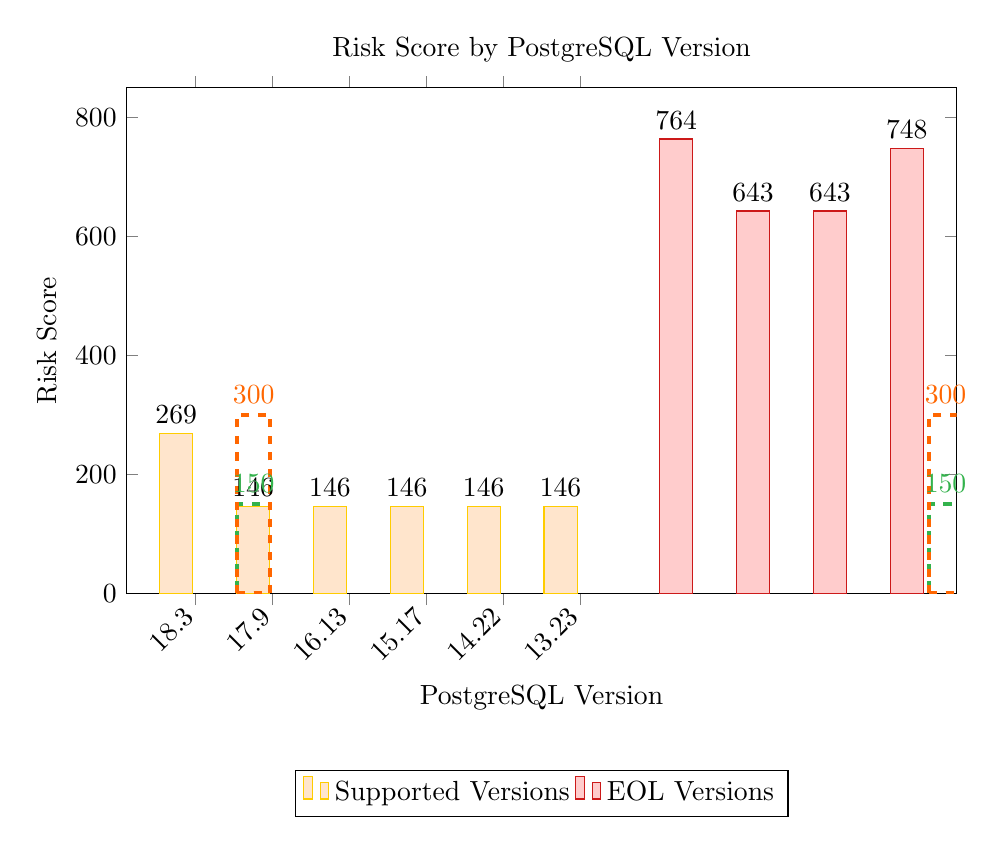
\begin{tikzpicture}
\begin{axis}[
    ybar,
    width=\textwidth,
    height=8cm,
    title={Risk Score by PostgreSQL Version},
    xlabel={PostgreSQL Version},
    ylabel={Risk Score},
    symbolic x coords={18.3, 17.9, 16.13, 15.17, 14.22, 13.23, 12.22, 11.22, 10.23, 9.6.24},
    xtick=data,
    x tick label style={rotate=45, anchor=east},
    nodes near coords,
    nodes near coords align={vertical},
    legend style={at={(0.5,-0.35)}, anchor=north, legend columns=3},
    ymin=0,
    ymax=850,
    enlarge x limits=0.1,
    bar width=12pt
]
\addplot[fill=lightorange, draw=vuln-medium] coordinates {(18.3,269) (17.9,146) (16.13,146) (15.17,146) (14.22,146) (13.23,146)};
\addplot[fill=lightred, draw=vuln-critical] coordinates {(12.22,764) (11.22,643) (10.23,643) (9.6.24,748)};

% Add risk level threshold lines
\addplot[color=gantt-supported, line width=1.5pt, dashed, forget plot] coordinates {(18.3,150) (9.6.24,150)};
\addplot[color=vuln-high, line width=1.5pt, dashed, forget plot] coordinates {(18.3,300) (9.6.24,300)};

\legend{Supported Versions, EOL Versions}
\end{axis}
\end{tikzpicture}
\caption{Risk scores showing dramatic security difference between supported (14-18) and EOL versions (9.6-13). Dashed lines indicate risk thresholds: Low Risk (below 150, green), Medium Risk (150-300, orange), High Risk (above 300, red).}
\label{fig:risk-score}
\end{figure}


\subsection{Critical CVE Examples}

To illustrate the concrete security risks of using unsupported versions, here are real critical vulnerabilities detected in PostgreSQL 12 (EOL November 2024):

\begin{table}[htbp]
\centering
\caption{Sample Critical CVEs in Unsupported Version (postgres:12)}
\label{tab:cve-examples}
\small
\begin{tabular}{@{}p{3cm}p{10cm}@{}}
\toprule
\textbf{CVE ID} & \textbf{Description} \\ \midrule
\href{https://nvd.nist.gov/vuln/detail/CVE-2025-15467}{CVE-2025-15467} & \textbf{OpenSSL}: Remote code execution or Denial of Service via oversized Initialization Vector in CMS parsing \\
\href{https://nvd.nist.gov/vuln/detail/CVE-2024-56171}{CVE-2024-56171} & \textbf{libxml2}: Use-After-Free vulnerability leading to potential remote code execution \\
\href{https://nvd.nist.gov/vuln/detail/CVE-2025-49794}{CVE-2025-49794} & \textbf{libxml}: Heap use-after-free (UAF) leads to Denial of Service (DoS) \\
\href{https://nvd.nist.gov/vuln/detail/CVE-2025-7458}{CVE-2025-7458} & \textbf{sqlite}: Integer overflow vulnerability enabling potential exploitation \\
\href{https://nvd.nist.gov/vuln/detail/CVE-2025-6965}{CVE-2025-6965} & \textbf{sqlite}: Integer truncation vulnerability in SQLite library \\
\bottomrule
\end{tabular}
\end{table}

\textbf{Key Takeaway:} These critical CVEs affect core dependencies (OpenSSL, libxml2, SQLite) bundled in the Docker image. Unsupported versions will never receive patches for these vulnerabilities, leaving systems permanently exposed.


\subsection{Version Lifecycle Timeline}

\begin{figure}[htbp]
\centering
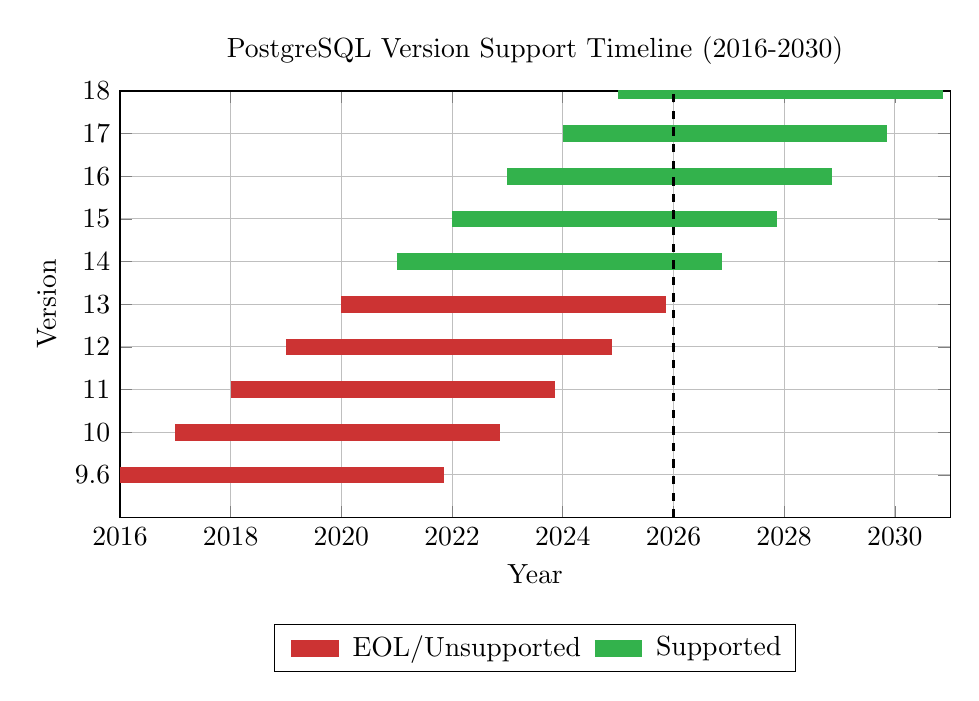
\begin{tikzpicture}
\begin{axis}[
    width=\textwidth,
    height=7cm,
    title={PostgreSQL Version Support Timeline (2016-2030)},
    xlabel={Year},
    ylabel={Version},
    xmin=2016, xmax=2031,
    ymin=0, ymax=10,
    ytick={1,2,3,4,5,6,7,8,9,10},
    yticklabels={9.6, 10, 11, 12, 13, 14, 15, 16, 17, 18},
    grid=major,
    legend style={at={(0.5,-0.25)}, anchor=north, legend columns=2},
    xticklabel style={/pgf/number format/set thousands separator={}}
]

% Unsupported versions (EOL periods)
\addplot[gantt-eol, line width=6pt] coordinates {(2016,1) (2021.86,1)}; % 9.6: 2016-2021.86
\addlegendentry{EOL/Unsupported}
\addplot[gantt-eol, line width=6pt, forget plot] coordinates {(2017,2) (2022.86,2)}; % 10: 2017-2022.86
\addplot[gantt-eol, line width=6pt, forget plot] coordinates {(2018,3) (2023.86,3)}; % 11: 2018-2023.86
\addplot[gantt-eol, line width=6pt, forget plot] coordinates {(2019,4) (2024.89,4)}; % 12: 2019-2024.89
\addplot[gantt-eol, line width=6pt, forget plot] coordinates {(2020,5) (2025.87,5)}; % 13: 2020-2025.87

% Supported versions
\addplot[gantt-supported, line width=6pt] coordinates {(2021,6) (2026.87,6)}; % 14: 2021-2026.87
\addlegendentry{Supported}
\addplot[gantt-supported, line width=6pt, forget plot] coordinates {(2022,7) (2027.87,7)}; % 15: 2022-2027.87
\addplot[gantt-supported, line width=6pt, forget plot] coordinates {(2023,8) (2028.86,8)}; % 16: 2023-2028.86
\addplot[gantt-supported, line width=6pt, forget plot] coordinates {(2024,9) (2029.86,9)}; % 17: 2024-2029.86
\addplot[gantt-supported, line width=6pt, forget plot] coordinates {(2025,10) (2030.87,10)}; % 18: 2025-2030.87

% Current date marker
\addplot[black, dashed, line width=1pt, forget plot] coordinates {(2026,0) (2026,10.5)};
\node at (axis cs:2026,10.5) [above] {\small Today};

\end{axis}
\end{tikzpicture}
\caption{PostgreSQL version support periods showing 5-year lifecycle policy. Supported versions shown in green, EOL versions in red.}
\label{fig:timeline}
\end{figure}


\subsection{Vulnerability Heat Map}

\begin{figure}[htbp]
\centering
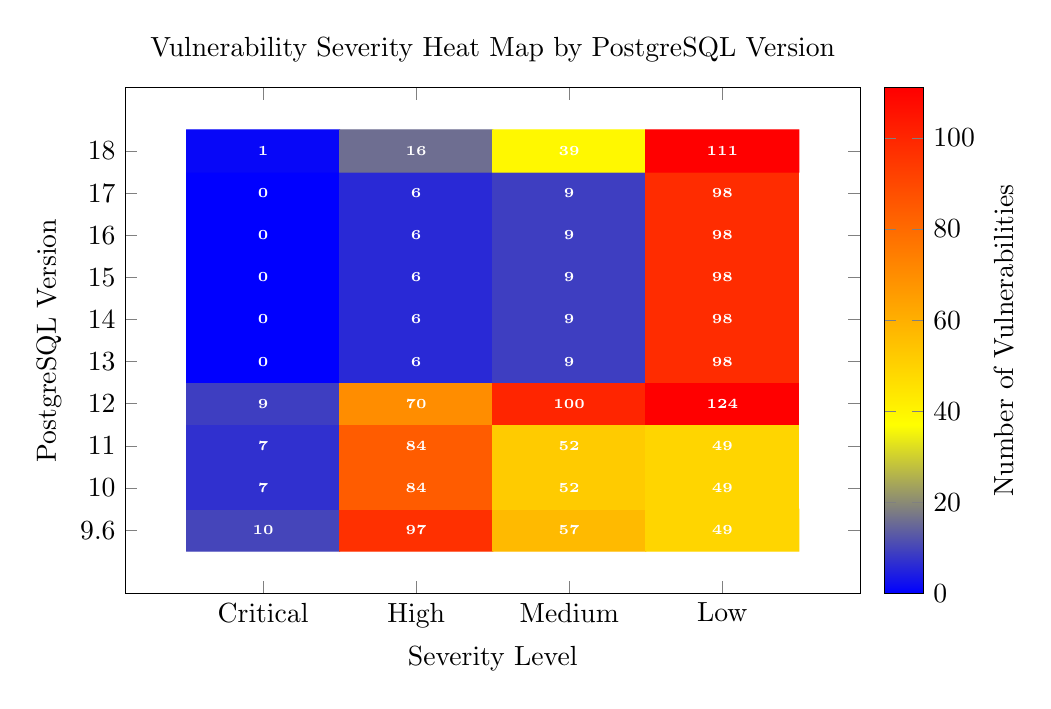
\begin{tikzpicture}
\begin{axis}[
    width=0.9\textwidth,
    height=8cm,
    title={Vulnerability Severity Heat Map by PostgreSQL Version},
    xlabel={Severity Level},
    ylabel={PostgreSQL Version},
    symbolic x coords={Critical, High, Medium, Low},
    symbolic y coords={9.6, 10, 11, 12, 13, 14, 15, 16, 17, 18},
    xtick=data,
    ytick=data,
    colormap/hot,
    colorbar,
    colorbar style={ylabel=Number of Vulnerabilities},
    point meta min=0,
    point meta max=111,
]

% Data points for heat map (version, severity, count)
\addplot[matrix plot*, mesh/cols=4, point meta=explicit] coordinates {
    (Critical,9.6)  [10]  (High,9.6)  [97]  (Medium,9.6)  [57]  (Low,9.6)  [49]
    (Critical,10)   [7]   (High,10)   [84]  (Medium,10)   [52]  (Low,10)   [49]
    (Critical,11)   [7]   (High,11)   [84]  (Medium,11)   [52]  (Low,11)   [49]
    (Critical,12)   [9]   (High,12)   [70]  (Medium,12)   [100] (Low,12)   [124]
    (Critical,13)   [0]   (High,13)   [6]   (Medium,13)   [9]   (Low,13)   [98]
    (Critical,14)   [0]   (High,14)   [6]   (Medium,14)   [9]   (Low,14)   [98]
    (Critical,15)   [0]   (High,15)   [6]   (Medium,15)   [9]   (Low,15)   [98]
    (Critical,16)   [0]   (High,16)   [6]   (Medium,16)   [9]   (Low,16)   [98]
    (Critical,17)   [0]   (High,17)   [6]   (Medium,17)   [9]   (Low,17)   [98]
    (Critical,18)   [1]   (High,18)   [16]  (Medium,18)   [39]  (Low,18)   [111]
};

% Add value labels with white text for better visibility on all cells
% Critical column
\node at (axis cs:Critical,9.6) [white] {\tiny\bf 10};
\node at (axis cs:Critical,10) [white] {\tiny\bf 7};
\node at (axis cs:Critical,11) [white] {\tiny\bf 7};
\node at (axis cs:Critical,12) [white] {\tiny\bf 9};
\node at (axis cs:Critical,13) [white] {\tiny\bf 0};
\node at (axis cs:Critical,14) [white] {\tiny\bf 0};
\node at (axis cs:Critical,15) [white] {\tiny\bf 0};
\node at (axis cs:Critical,16) [white] {\tiny\bf 0};
\node at (axis cs:Critical,17) [white] {\tiny\bf 0};
\node at (axis cs:Critical,18) [white] {\tiny\bf 1};

% High column
\node at (axis cs:High,9.6) [white] {\tiny\bf 97};
\node at (axis cs:High,10) [white] {\tiny\bf 84};
\node at (axis cs:High,11) [white] {\tiny\bf 84};
\node at (axis cs:High,12) [white] {\tiny\bf 70};
\node at (axis cs:High,13) [white] {\tiny\bf 6};
\node at (axis cs:High,14) [white] {\tiny\bf 6};
\node at (axis cs:High,15) [white] {\tiny\bf 6};
\node at (axis cs:High,16) [white] {\tiny\bf 6};
\node at (axis cs:High,17) [white] {\tiny\bf 6};
\node at (axis cs:High,18) [white] {\tiny\bf 16};

% Medium column
\node at (axis cs:Medium,9.6) [white] {\tiny\bf 57};
\node at (axis cs:Medium,10) [white] {\tiny\bf 52};
\node at (axis cs:Medium,11) [white] {\tiny\bf 52};
\node at (axis cs:Medium,12) [white] {\tiny\bf 100};
\node at (axis cs:Medium,13) [white] {\tiny\bf 9};
\node at (axis cs:Medium,14) [white] {\tiny\bf 9};
\node at (axis cs:Medium,15) [white] {\tiny\bf 9};
\node at (axis cs:Medium,16) [white] {\tiny\bf 9};
\node at (axis cs:Medium,17) [white] {\tiny\bf 9};
\node at (axis cs:Medium,18) [white] {\tiny\bf 39};

% Low column
\node at (axis cs:Low,9.6) [white] {\tiny\bf 49};
\node at (axis cs:Low,10) [white] {\tiny\bf 49};
\node at (axis cs:Low,11) [white] {\tiny\bf 49};
\node at (axis cs:Low,12) [white] {\tiny\bf 124};
\node at (axis cs:Low,13) [white] {\tiny\bf 98};
\node at (axis cs:Low,14) [white] {\tiny\bf 98};
\node at (axis cs:Low,15) [white] {\tiny\bf 98};
\node at (axis cs:Low,16) [white] {\tiny\bf 98};
\node at (axis cs:Low,17) [white] {\tiny\bf 98};
\node at (axis cs:Low,18) [white] {\tiny\bf 111};

\end{axis}
\end{tikzpicture}
\caption{Heat map visualization showing vulnerability counts by severity and version. Darker colors indicate higher vulnerability counts.}
\label{fig:heatmap}
\end{figure}


\subsection{Cost-Benefit Analysis: Upgrade vs. Risk}

\begin{table}[htbp]
\centering
\caption{Upgrade Effort vs. Security Risk Assessment}
\label{tab:cost-benefit}
\begin{tabular}{@{}lccp{6cm}@{}}
\toprule
\textbf{Migration Path} & \textbf{Effort} & \textbf{Risk Reduction} & \textbf{Notes} \\ \midrule
\rowcolor{lightgreen} 13 $\rightarrow$ 14 & Low & High & Single major version jump, similar features \\
\rowcolor{lightgreen} 12 $\rightarrow$ 14 & Medium & Very High & 2 major versions, eliminates 9 critical CVEs \\
\rowcolor{lightorange} 11 $\rightarrow$ 15 & Medium & Very High & 4 major versions, significant feature changes \\
\rowcolor{lightred} 10 $\rightarrow$ 16 & High & Critical & 6 major versions, requires thorough testing \\
\rowcolor{lightred} 9.6 $\rightarrow$ 17/18 & Very High & Critical & 8-9 major versions, extensive compatibility review needed \\
\bottomrule
\end{tabular}
\end{table}

\textbf{Recommendation Strategy:}
\begin{itemize}
    \item \textbf{Step 1:} Upgrade to the minimum supported version (14) immediately to escape EOL status
    \item \textbf{Step 2:} Plan migration to version 16 or 17 for long-term support (EOL 2028-2029)
    \item \textbf{Step 3:} Establish regular minor update process to stay current within major version
\end{itemize}


\subsection{Vulnerability Comparison: 18.0 vs 18.1 vs 18.2 vs 18.3}
\label{subsec:patch-comparison}

To illustrate the importance of patch releases, we compare the vulnerabilities found in \texttt{postgres:18} versions.

\begin{table}[htbp]
\centering
\caption{Vulnerability Comparison: PostgreSQL 18.0 vs 18.1 vs 18.2 vs 18.3 with Risk Scores}
\label{tab:trivy-compare}
\begin{tabular}{@{}lcccccc@{}}
	\textbf{Docker Tag} & \textbf{Critical} & \textbf{High} & \textbf{Medium} & \textbf{Low} & \textbf{Total} & \textbf{Risk Score} \\ \midrule
\rowcolor{lightorange} \texttt{postgres:18.0} & 4 & 30 & 68 & 102 & 204 & \textbf{428} \\
\rowcolor{lightorange} \texttt{postgres:18.1} & 1 & 17 & 39 & 102 & 159 & \textbf{275} \\
\rowcolor{lightorange} \texttt{postgres:18.2} & 1 & 16 & 39 & 111 & 167 & \textbf{269} \\
\rowcolor{lightorange} \texttt{postgres:18.3} & 1 & 16 & 39 & 111 & 167 & \textbf{269} \\
\bottomrule
\end{tabular}
\end{table}

\begin{tcolorbox}[colback=lightorange!20, colframe=vuln-high, title=📊 Patch Release Value: 18.0 → 18.3 Analysis, fonttitle=\bfseries]
The upgrade from 18.0 to 18.3 delivered immediate security improvements:
\begin{itemize}
    \item \textbf{75\% reduction} in critical CVEs (4 → 1)
    \item \textbf{47\% reduction} in high-severity issues (30 → 16)
    \item \textbf{18\% overall reduction} in total vulnerabilities (204 → 167)
    \item \textbf{37\% reduction} in risk score (428 → 269) - from High to Medium risk
\end{itemize}
\textbf{Note:} PostgreSQL 18.2 and 18.3 have identical vulnerability profiles, indicating stable security posture.\\
\textbf{Recommendation:} Always deploy the latest patch within your chosen major version.
\end{tcolorbox}

\begin{figure}[htbp]
\centering
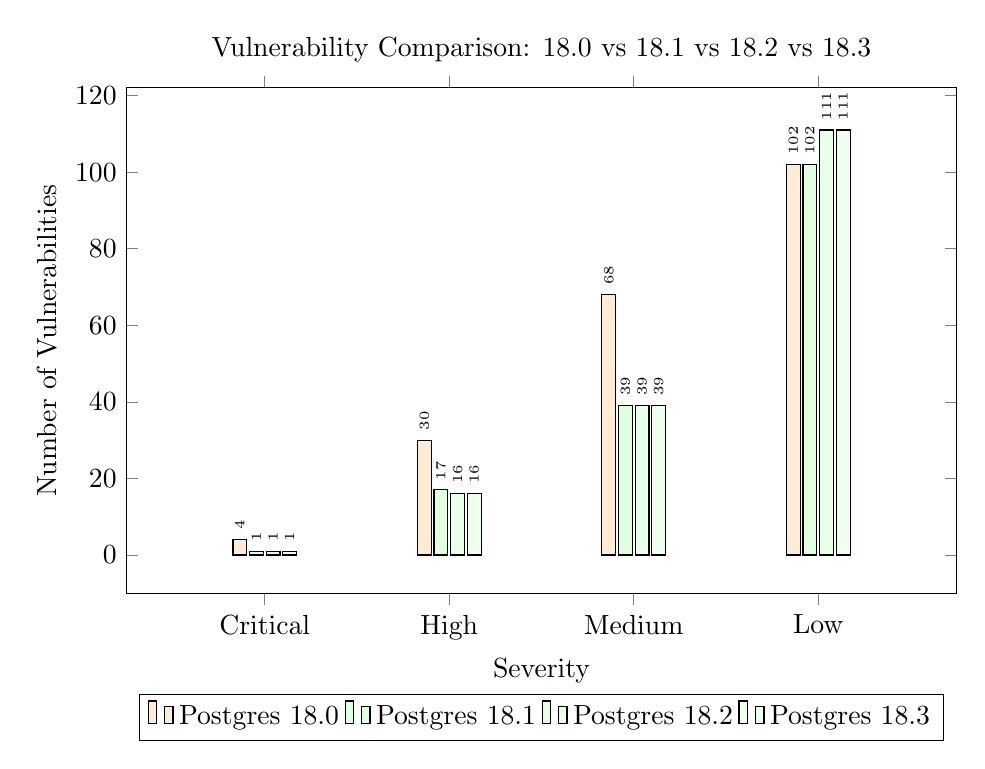
\begin{tikzpicture}
\begin{axis}[
    ybar=1pt,
    bar width=5pt,
    width=\textwidth,
    height=8cm,
    title={Vulnerability Comparison: 18.0 vs 18.1 vs 18.2 vs 18.3},
    xlabel={Severity},
    ylabel={Number of Vulnerabilities},
    symbolic x coords={Critical, High, Medium, Low},
    xtick=data,
    nodes near coords,
    nodes near coords align={vertical},
    every node near coord/.append style={rotate=90, anchor=west, font=\tiny},
    legend style={at={(0.5,-0.2)}, anchor=north, legend columns=4},
    enlarge x limits=0.25
]
\addplot[fill=lightorange!80] coordinates {(Critical,4) (High,30) (Medium,68) (Low,102)};
\addplot[fill=lightgreen!80] coordinates {(Critical,1) (High,17) (Medium,39) (Low,102)};
\addplot[fill=lightgreen!60] coordinates {(Critical,1) (High,16) (Medium,39) (Low,111)};
\addplot[fill=lightgreen!40] coordinates {(Critical,1) (High,16) (Medium,39) (Low,111)};
\legend{Postgres 18.0, Postgres 18.1, Postgres 18.2, Postgres 18.3}
\end{axis}
\end{tikzpicture}
\caption{Comparison of vulnerabilities detected by \texttt{trivy} for PostgreSQL 18.0-18.3. Grouped bars show clear reduction in critical and high severity issues from 18.0 to 18.1. Versions 18.2 and 18.3 maintain identical security profiles.}
\label{fig:vuln-chart-18.0-18.1}
\end{figure}

The updates from 18.0 to 18.3 significantly reduced the number of critical and high vulnerabilities, with the most dramatic improvements occurring in the 18.0 → 18.1 transition. PostgreSQL 18.2 and 18.3 maintain identical vulnerability counts, demonstrating a stabilized security posture. For detailed changes, refer to the respective changelogs: \href{https://www.postgresql.org/docs/18/release-18.html}{18.0}, \href{https://www.postgresql.org/docs/18/release-18-1.html}{18.1}, \href{https://www.postgresql.org/docs/18/release-18-2.html}{18.2}, and \href{https://www.postgresql.org/docs/18/release-18-3.html}{18.3}.

\subsection{Docker Image Metadata: Ensuring Reproducible Scans}
\label{subsec:docker-metadata}

When performing security scans, it's crucial to understand that Docker tags like \texttt{postgres:18} are mutable references that can point to different images over time. For reproducible vulnerability scans and audit trails, we use \textbf{manifest digests} (SHA256 hashes) to reference specific image builds.

\subsubsection{Understanding Docker Image Identifiers}

Docker images can be referenced in three ways:
\begin{itemize}
    \item \textbf{Tag}: \texttt{postgres:18.3} (mutable, points to latest patch)
    \item \textbf{Manifest Digest}: \texttt{sha256:eb37f5864...} (immutable, specific build)
    \item \textbf{Digest Reference}: \texttt{postgres:18.3@sha256:eb37f5864...} (tag + digest for clarity)
\end{itemize}

\subsubsection{PostgreSQL 18.x Image Digests}

The following table documents the exact Docker Hub manifest digests used for vulnerability analysis in this report:

\begin{table}[htbp]
\centering
\caption{Docker Hub Manifest Digests for PostgreSQL 18.x Images}
\label{tab:docker-digests}
\small
\begin{tabular}{@{}lp{5.5cm}l@{}}
\toprule
\textbf{Tag} & \textbf{Manifest Digest (SHA256)} & \textbf{Architecture} \\ \midrule
\texttt{postgres:18.0} & \texttt{192a387c...ebb3aed} & linux/amd64 \\
\texttt{postgres:18.1} & \texttt{2ccc3d98...07395abc} & linux/amd64 \\
\texttt{postgres:18.2} & \texttt{79aafbb6...f0a641e2} & linux/amd64 \\
\texttt{postgres:18.3} & \texttt{5aa97b30...bd458326d} & linux/amd64 \\
\bottomrule
\end{tabular}
\end{table}

\subsubsection{Docker Hub Image URIs}

For complete transparency and auditability, the full Docker Hub layer URLs for each release:

\begin{itemize}
    \item \textbf{18.0}: \href{https://hub.docker.com/layers/library/postgres/18.0/images/sha256-192a387c789cac29fcc7ac9a3a99060642a052fa293fd1953954c0956ebb3aed}{hub.docker.com/.../sha256-192a387...}
    \item \textbf{18.1}: \href{https://hub.docker.com/layers/library/postgres/18.1/images/sha256-2ccc3d98b960df5ed1ee2d32d3d5338a3c688cf899c0e951ce6d45fb07395abc}{hub.docker.com/.../sha256-2ccc3d9...}
    \item \textbf{18.2}: \href{https://hub.docker.com/layers/library/postgres/18.2/images/sha256-79aafbb673bb55e26ca128ec4d68b5ec30de64175c6d13f3eff29651f0a641e2}{hub.docker.com/.../sha256-79aafbb...}
    \item \textbf{18.3}: \href{https://hub.docker.com/layers/library/postgres/18.3/images/sha256-e47309bc9a186ae58078b35a385dc89216d922c0f2f5cbb2bd6390e878dce27e}{hub.docker.com/.../sha256-e47309bc9...}
\end{itemize}

\subsubsection{Scanning with Digest References}

To scan a specific image build regardless of tag updates:

\begin{verbatim}
trivy image postgres@sha256:eb37f58646a901dc7727cf448cae36d...
\end{verbatim}

Or with both tag and digest for documentation:

\begin{verbatim}
trivy image postgres:18.3@sha256:eb37f58646a901dc7727cf448...
\end{verbatim}

\begin{tcolorbox}[colback=lightorange!20, colframe=vuln-high, title=⚠️ Important: Image Digest Best Practices, fonttitle=\bfseries]
\textbf{Why Digests Matter:}
\begin{itemize}
    \item Tags can be overwritten - \texttt{postgres:18} may point to different images over time
    \item Digests are immutable - \texttt{sha256:eb37f58...} always references the exact same layers
    \item CI/CD pipelines should pin digests for reproducible builds
    \item Security audits require digest tracking for compliance and forensics
    \item Base image updates may silently change vulnerability profiles when using tags
\end{itemize}
\end{tcolorbox}

\subsubsection{Verifying Image Digests}

To verify the current digest of a tagged image:

\begin{verbatim}
docker inspect postgres:18.3 --format='{{.RepoDigests}}'
\end{verbatim}

Or using \texttt{crane} (Google's container tool):

\begin{verbatim}
crane digest postgres:18.3
\end{verbatim}

This verification step ensures your local image matches the documented digest used in this analysis.


\section{Recommendations}
\label{sec:recommendations}

Based on the comprehensive security analysis presented in this report, the following actions are recommended:

\subsection{Migration Impact: Before \& After}

To illustrate the concrete security benefits of upgrading, here's a comparison of migrating from an EOL version to a supported version:

\begin{table}[htbp]
\centering
\caption{Security Impact of Upgrading from PostgreSQL 12 to 17}
\label{tab:before-after}
\begin{tabular}{@{}lcc@{}}
\toprule
\textbf{Metric} & \textbf{Before (v12)} & \textbf{After (v17)} \\ \midrule
\rowcolor{lightred} Critical CVEs & 9 & 0 \\
\rowcolor{lightorange} High CVEs & 70 & 6 \\
\rowcolor{lightorange} Medium CVEs & 100 & 9 \\
\rowcolor{lightgreen} Low CVEs & 124 & 98 \\
\midrule
\textbf{Total Vulnerabilities} & \textbf{305} & \textbf{113} \\
\rowcolor{lightorange} \textbf{Risk Score} & \textbf{764 (High)} & \textbf{146 (Low)} \\
\rowcolor{lightgreen} \textbf{Vulnerability Reduction} & - & \textbf{63\%} \\
\rowcolor{lightgreen} \textbf{Risk Score Reduction} & - & \textbf{81\%} \\
\rowcolor{lightgreen} Support Status & \textbf{EOL'd (Nov 2024)} & \textbf{Supported until Nov 2029} \\
\bottomrule
\end{tabular}
\end{table}

\begin{tcolorbox}[colback=lightgreen!20, colframe=gantt-supported, title=💡 Business Case for Migration, fonttitle=\bfseries]
Upgrading from PostgreSQL 12 to 17 eliminates \textbf{all 9 critical vulnerabilities}, reduces the risk score from \textbf{764 (High Risk) to 146 (Low Risk)} - an \textbf{81\% reduction}, and provides \textbf{5 years of continued support}. The security ROI is immediate and substantial.
\end{tcolorbox}

\subsection{Immediate Actions (Critical Priority)}

\begin{itemize}
    \item \textbf{Migrate from EOL Versions:} If currently running PostgreSQL versions $\leq$13, plan immediate migration to version $\geq$14. These versions contain 2-10$\times$ more vulnerabilities.
    \item \textbf{Audit Current Deployments:} Use \texttt{geol check} command to continuously monitor PostgreSQL lifecycle status. Run \texttt{geol help check} for more information.
    \item \textbf{Scan Docker Images:} Integrate \texttt{trivy image postgres:X --severity CRITICAL,HIGH} into deployment workflows.
\end{itemize}

\subsection{Long-Term Strategy}

\begin{itemize}
    \item \textbf{Target Version Selection:}
    \begin{itemize}
        \item Minimum: PostgreSQL 14 (EOL Nov 2026) - escape EOL status
        \item Recommended: PostgreSQL 16-17 (EOL 2028-2029) - optimal support window
        \item Latest: PostgreSQL 18 (EOL Nov 2030) - maximum future-proofing
    \end{itemize}
    \item \textbf{Patch Management:} Establish automated monitoring for minor releases - as shown in Section \ref{subsec:patch-comparison}, patches can reduce vulnerabilities by 22\% or more.
    \item \textbf{Docker Tag Strategy:} Use specific version tags (e.g., \texttt{postgres:17.7}) instead of major version tags to control updates.
\end{itemize}

\subsection{DevSecOps Integration}

\begin{itemize}
    \item Implement automated EOL checking in quality gates
    \item Set up vulnerability scanning as a deployment prerequisite
    \item Schedule quarterly reviews of PostgreSQL version lifecycle status
    \item Document upgrade paths and maintain rollback procedures
\end{itemize}

\section{Summary and conclusion}

The combined data analysis is clear. Figure \ref{fig:vuln-chart} strikingly illustrates this divergence:

\begin{itemize}
    \item \textbf{The danger of unsupported versions:} Versions that have reached their end of life (12, 11, 10, 9.6) accumulate a dangerous number of vulnerabilities, including several \textbf{critical} ones.
    \item \textbf{The security of supported versions:} In contrast, images of maintained versions (14 to 18) show no critical vulnerabilities and a low, consistent risk profile. Note that PostgreSQL 13 is now unsupported.
    \item \textbf{Recommendation:} The choice of PostgreSQL version must be for an actively supported version. The security risk of using an obsolete version is real and high.\\
\end{itemize}

Tools like \texttt{geol} and \texttt{trivy} are essential in a modern DevSecOps approach. This analysis of PostgreSQL perfectly illustrates how abandoning software support directly leads to a drastic increase in security flaws. Using up-to-date versions is not just a recommendation, but a necessity for the security of any infrastructure.

\section{Resources}

\begin{multicols}{2}
\begin{itemize}
    \item \href{https://dev.to/adriens/geol-the-cli-to-efficiently-manage-eols-like-a-boss-3hne}{geol, the cli to efficiently manage EOLs like a boss}
    \item \href{https://youtu.be/ZqiXogK2fSw}{geol - Gérer la fin de vie (notebookLM slideshow) v1.3.0 - "for dummies" edition}
    \item \href{https://youtu.be/yCZRgAiQt9s}{geol 1.3.0 unboxing - the check command}
    \item \href{https://youtu.be/vhFXWGqB_-g}{MVP Unboxing geol - a devops secops cli to manage EOLs and product lifecycle}
    \item \href{https://github.com/adriens/geol-showcase}{geol-showcase, A set of resources to showcase what could be achieved with geol, datascience, AI and devsecops tools}
    \item \href{https://www.postgresql.org/about/news/postgresql-181-177-1611-1515-1420-and-1323-released-3171/}{PostgreSQL 18.1, 17.7, 16.11, 15.15, 14.20, and 13.23 Released!}
    \item \href{https://endoflife.date/postgresql}{PostgreSQL EOL Data}
\end{itemize}
\end{multicols}

\end{document}
